
% This LaTeX was auto-generated from an M-file by MATLAB.
% To make changes, update the M-file and republish this document.

\documentclass{article}
\usepackage{graphicx}
\usepackage{color}

\sloppy
\definecolor{lightgray}{gray}{0.5}
\setlength{\parindent}{0pt}

\begin{document}



\subsection*{Contents - With restarted GMRES}

\begin{itemize}
\setlength{\itemsep}{-1ex}
   \item Jacobi
   \item BLKJacobi
   \item GS
   \item SOR
   \item GMRES-100
   \item PGMRES-100
   \item Plotting commands
\end{itemize}
\begin{verbatim}
function A1q3()
\end{verbatim}
\begin{verbatim}
close all
clc

sigma = -10;
tau = -20;
n = 2^10;
h = 1/(n+1);

beta = sigma*h/2;
gamma = tau*h/2;
fprintf('\n    =====================================================')
fprintf('\n      Solving the Convection-Diffusion equation with\n')
fprintf('         beta = %2.4f, gamma = %2.4f and n = %3i\n',beta,gamma,n)
fprintf('    =====================================================\n')
% Creating discretised Convection Diffusion matrix
A = ConvectionDiffusion(beta,gamma,n);

% Defin exact solution and RHS functions
u = @(x,y) sin(pi*x).*cos(pi*y);
f = @(x,y,sigma,tau) 2*pi^2*u(x,y)+sigma*pi*cos(pi*x).*cos(pi*y) ...
    -tau*pi*sin(pi*x).*sin(pi*y);

% Creating domain
x = linspace(0,1,n+2);
[X,Y] = meshgrid(x,x);


% Defining RHS vector
F = f(X,Y,sigma,tau);
% Applying  Dirichlet boundary conditions
F(:,1) = sparse(n+2,1);
F(:,end) = sparse(n+2,1);
F = h^2*F(:);

% Defining exact solution
uE = u(X,Y);
uE = uE(:);

% Calculating error
tic
uA = A\F;
Dtime = toc;
fprintf('\n      Time using backslash = %4.4f',Dtime)
fprintf('\n      solution norm = %1.4e \n\n\n',norm(uE-uA,inf));

% Setting up initial guess
x = sparse((n+2)^2,1);

% Defining iterative parameters
max_iter = 2000;
tol = 1e-6;
\end{verbatim}

        \color{lightgray} \begin{verbatim}
    =====================================================
      Solving the Convection-Diffusion equation with
         beta = -0.0049, gamma = -0.0098 and n = 1024
    =====================================================

      Time using backslash = 12.1265
      solution norm = 1.5935e-06


\end{verbatim} \color{black}


\subsection*{Jacobi}

\begin{verbatim}
[~,rJ,iterJ] = Jacobi(max_iter,tol,x,A,F);
\end{verbatim}

        \color{lightgray} \begin{verbatim}                      ------------------
                      |     Jacobi     |
                      ------------------
      Residual after error 2000 interations = 3.4810e-02
      Time to run Jacobi = 51.6430

\end{verbatim} \color{black}


\subsection*{BLKJacobi}

\begin{verbatim}
[~,rBLK,iterBLK] = BLKJacobi(max_iter,tol,x,A,F);
\end{verbatim}

        \color{lightgray} \begin{verbatim}                      ------------------
                      |   BLK Jacobi   |
                      ------------------
      Residual after error 2000 interations = 3.4290e-02
      Time to run Jacobi = 125.7144

\end{verbatim} \color{black}


\subsection*{GS}

\begin{verbatim}
[~,rGS,iterGS] = GS(max_iter,tol,x,A,F);
\end{verbatim}

        \color{lightgray} \begin{verbatim}                      ------------------
                      |  Gauss-Siedel  |
                      ------------------
      Residual after error 2000 interations = 3.4316e-02
      Time to run GS = 82.9518

\end{verbatim} \color{black}


\subsection*{SOR}

\begin{verbatim}
fprintf('                      ------------------     \n');
fprintf('                      |      SOR       |   \n');
fprintf('                      ------------------     \n');
ii = 0;
rSOR = cell(9,1);
iterSOR = sparse(9,1);
test = zeros(9,1);
omega = zeros(9,1);
for i = 1.1:.1:1.9
    ii = ii + 1;
    [~,rSORR,iterSOR(ii)] = SOR(max_iter,tol,x,A,F,i);
    rSOR{ii} = rSORR;
    test(ii) = rSORR(end);
    omega(ii) = i;
end
[~,index]=min(test);
\end{verbatim}

        \color{lightgray} \begin{verbatim}                      ------------------
                      |      SOR       |
                      ------------------
      Omega = 1.1
      Residual after error 2000 interations = 3.4113e-02
      Time to run SOR = 92.3514

      Omega = 1.2
      Residual after error 2000 interations = 3.3869e-02
      Time to run SOR = 103.5740

      Omega = 1.3
      Residual after error 2000 interations = 3.3570e-02
      Time to run SOR = 107.5515

      Omega = 1.4
      Residual after error 2000 interations = 3.3190e-02
      Time to run SOR = 106.1925

      Omega = 1.5
      Residual after error 2000 interations = 3.2686e-02
      Time to run SOR = 116.8397

      Omega = 1.6
      Residual after error 2000 interations = 3.1975e-02
      Time to run SOR = 105.1813

      Omega = 1.7
      Residual after error 2000 interations = 3.0874e-02
      Time to run SOR = 106.0727

      Omega = 1.8
      Residual after error 2000 interations = 2.8888e-02
      Time to run SOR = 105.2235

      Omega = 1.9
      Residual after error 2000 interations = 2.3957e-02
      Time to run SOR = 103.5844

\end{verbatim} \color{black}


\subsection*{GMRES-100}

\begin{verbatim}
tic
[~,~,~,iterGM,rGM] = gmres(A,F,[100],tol,max_iter);
time = toc;
% Produces results
fprintf('                      -----------------     \n');
fprintf('                      |  GMRES-100    |   \n');
fprintf('                      -----------------     \n');
fprintf('      Residual error after %4.0f %4.0f inner and outter interations = %1.4e \n'...
    ,iterGM(1),iterGM(end),rGM(end))
fprintf('      Time to run CG = %2.4f\n\n',time)
\end{verbatim}

        \color{lightgray} \begin{verbatim}                      -----------------
                      |  GMRES-100    |
                      -----------------
      Residual error after   79   37 inner and outter interations = 3.5575e-08
      Time to run CG = 10156.5268

\end{verbatim} \color{black}


\subsection*{PGMRES-100}

\begin{verbatim}
tic
setup.type = 'nofill';
[L,U] = ilu(A,setup);
[~,~,~,iterPGM,rPGM] = gmres(A,F,[100],tol,max_iter,L,U);
time = toc;
% Produces results
fprintf('                      -----------------     \n');
fprintf('                      |  PGMRES-100   |   \n');
fprintf('                      -----------------     \n');
fprintf('      Residual error after %4.0f %4.0f inner and outter interations = %1.4e \n'...
    ,iterPGM(1),iterPGM(end),rPGM(end))
fprintf('      Time to run CG = %2.4f\n\n',time)

rSOR = rSOR{index};
m_iter = max([iterJ,iterBLK,iterGS,iterSOR(index),sum(iterGM),sum(iterPGM)]);
m_res = max([rJ(1),rBLK(1),rGS(1),rSOR(1),rGM(1),rPGM(1)]);
\end{verbatim}

        \color{lightgray} \begin{verbatim}                      -----------------
                      |  PGMRES-100   |
                      -----------------
      Residual error after   20   59 inner and outter interations = 6.0384e-08
      Time to run CG = 2749.8409

\end{verbatim} \color{black}


\subsection*{Plotting commands}

\begin{verbatim}
semilogy(rJ,'c'); hold on
semilogy(rBLK,'k'); hold on
semilogy(rGS,'r--');hold on
semilogy(rSOR,'b-.');hold on
semilogy(rGM,'g');hold on
semilogy(rPGM,'c--');hold on
axis([0 m_iter tol m_res]);
legend('Jacobi','block Jacobi','GS',['SOR-omega=',num2str(omega(index))]...
    ,'GMRES','GMRES-ilu','Location','Best')
xlabel('Iterations','fontsize',14);
ylabel('Residual error','fontsize',14);
\end{verbatim}

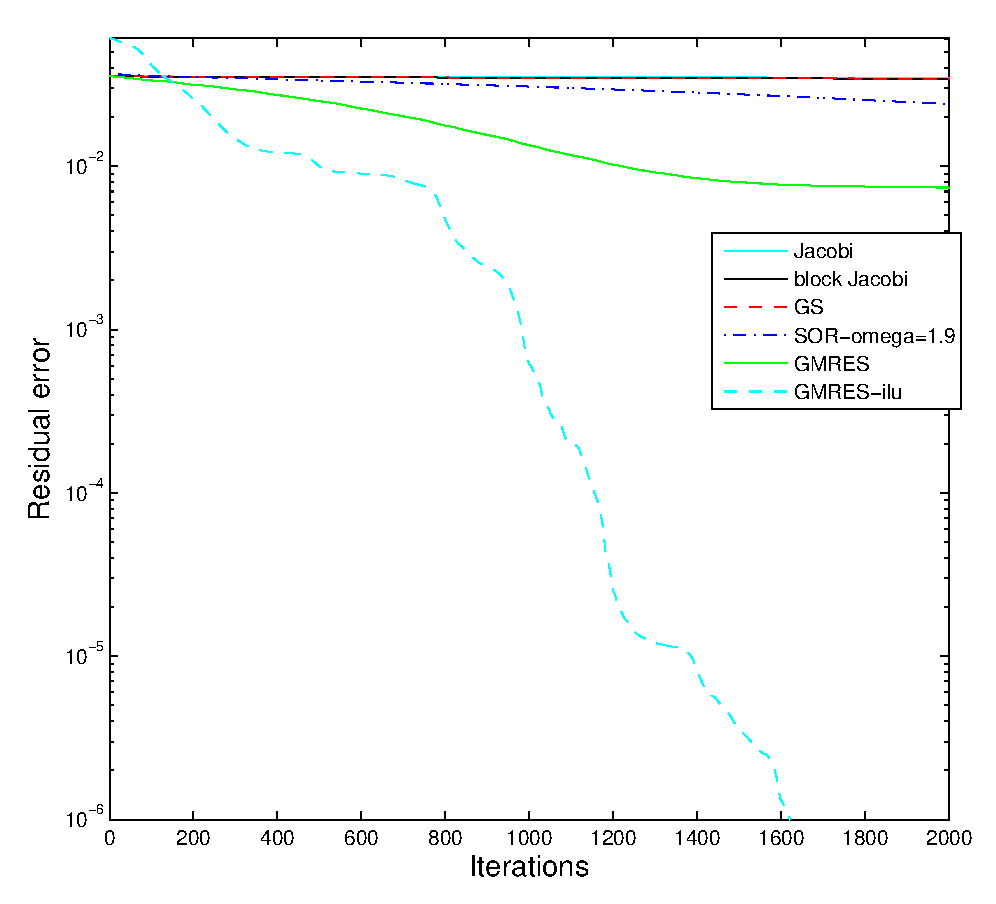
\includegraphics [width=4in]{A1q3_01restart.eps}
\begin{verbatim}
    function [A] = ConvectionDiffusion(beta,gamma,n)

        e = ones(n,1);

        % Creating sparse diagonal matrices
        I = spdiags(e,0,n,n);
        I1 =spdiags(e,1,n,n);
        I2 = spdiags(e,-1,n,n);

        % Creating 1D Convection-Diffusion matricies
        Abeta = 2*I +(beta-1)*I1 - (beta+1)*I2;
        Agamma = 2*I +(gamma-1)*I1 - (gamma+1)*I2;

        % applying boundary conditions
        AbetaBC = [1 sparse(1,n+1);[-(beta+1); sparse(n-1,1)] ...
            Abeta [sparse(n-1,1); beta-1];sparse(1,n+1) 1];
        AgammaBC = [2 -2 sparse(1,n);[-(gamma+1); sparse(n-1,1)]...
            Agamma [sparse(n-1,1); gamma-1];sparse(1,n) -2 2 ];

        % Creating 2D Convection-Diffusion matrix
        A = kron(AbetaBC,speye(n+2))+kron(speye(n+2),AgammaBC);

    end


    function [x,rJ,i] = Jacobi(max_iter,tol,x,A,b)
        % Jacobi method
        tic
        % Creating vector of diagonals of A
        D = spdiags(A,0);
        b_norm = norm(b);
        r = b;

        % Carring out Jacobi
        for i = 1:max_iter

            % updating x
            x = x + r./D;
            r = b-A*x;
            rJ(i) = norm(r);

            if (rJ(i)/b_norm) < tol
                break
            end
        end
        time = toc;
        % Produces results
        fprintf('                      ------------------     \n');
        fprintf('                      |     Jacobi     |   \n');
        fprintf('                      ------------------     \n');
        fprintf('      Residual after error %4.0f interations = %1.4e \n'...
            ,i,rJ(i))
        fprintf('      Time to run Jacobi = %2.4f\n\n',time)
    end


    function [x,rJ,i] = BLKJacobi(max_iter,tol,x,A,b)
        % Jacobi method
        tic
        % Creating Block Jacobi
        BLKjac = spdiags([spdiags(A,-1),spdiags(A,0),spdiags(A,1)]...
            ,[-1:1],(n+2)^2,(n+2)^2);
        b_norm = norm(b);
        r = b;
        % Factoring BLKjac so can use backwards and forwards subsitution at
        % each step
        [LowT,UpT,Piv] = lu(BLKjac,'vector');
        % Carring out BLKJacobi
        for i = 1:max_iter

            % updating x
            x = x + UpT\(LowT\(r(Piv,:)));

            r = b-A*x;
            rJ(i) = norm(r);

            if (rJ(i)/b_norm) < tol
                break
            end
        end
        time = toc;
        % Produces results
        fprintf('                      ------------------     \n');
        fprintf('                      |   BLK Jacobi   |   \n');
        fprintf('                      ------------------     \n');
        fprintf('      Residual after error %4.0f interations = %1.4e \n'...
            ,i,rJ(i))
        fprintf('      Time to run Jacobi = %2.4f\n\n',time)
    end

    function [x,rGS,i] = GS(max_iter,tol,x,A,b)
        tic
        % Creating lower triangular
        E = tril(A);
        b_norm = norm(b);
        r = b;

        % Carring out GS
        for i = 1:max_iter

            % updating x
            x = x + E\r;
            r = b-A*x;
            rGS(i) = norm(r);

            if (rGS(i)/b_norm) < tol
                break
            end
        end
        time = toc;
        % Produces results
        fprintf('                      ------------------     \n');
        fprintf('                      |  Gauss-Siedel  |   \n');
        fprintf('                      ------------------     \n');
        fprintf('      Residual after error %4.0f interations = %1.4e \n'...
            ,i,rGS(i))
        fprintf('      Time to run GS = %2.4f\n\n',time)
    end


    function [x,rSOR,i] = SOR(max_iter,tol,x,A,b,omega)
        tic
        % Creating lower triangular
        E = tril(A);
        [N,~] = size(A);
        % Creating sparse diagonal matrix
        D = spdiags(spdiags(A,0),0,N,N);

        % Calculating the matrix which we need to solve at each step
        S = ((1/omega-1)*D+E);
        b_norm = norm(b);
        r = b;

        % Carring out SOR
        for i = 1:max_iter

            % updating x
            x = x + S\r;
            r = b-A*x;
            rSOR(i) = norm(r);

            if (rSOR(i)/b_norm) < tol
                break
            end
        end
        time = toc;
        % Produces results
        fprintf('      Omega = %1.1f \n',omega)
        fprintf('      Residual after error %4.0f interations = %1.4e \n'...
            ,i,rSOR(i))
        fprintf('      Time to run SOR = %2.4f\n\n',time)
    end
\end{verbatim}
\begin{verbatim}
end
\end{verbatim}



\end{document}

